% Конкретные численные значения, которые использовались (входные данные)
\subsection*{Исходные данные экспериментальной модели}
В целях исследования безотказности работы сформированной модели и сложности ее анализа различными решателями проводился ряд экспериментов. В качестве входных данных для разных решателей использовалась сформированная ранее модель. Такая модель позволяет применять решатели по открытой лицензии.
Характеристики оборудования, используемого для проведения экспериментов:
\begin{itemize}
  \item операционная система - Ubuntu 23.04;
  \item процессор - 2-ядерный процессор Intel Core i5 с тактовой частотой 1,8GHz;
  \item объем ОЗУ - 8 ГБ.
\end{itemize}

% Таблица с применением решателей для решения моей сформированной модели
\subsection*{Результаты экспериментов}
Экспериментальная модель была обсчитана рядом решателей: \textit{glpk}, \textit{gurobi}, \textit{xpress}, \textit{gams}, \textit{gdpopt}, \textit{mindtpy}, \textit{cbc}, \textit{conopt}, \textit{copt}, \textit{cplex}, \textit{ilogcp} и \textit{minos}.

В рамках проведения экспериментов каждый решатель обсчитал модель по $100$ раз. При каждом обсчете замерялось время, необходимое решателю для выполнения вычислений, а так же результирующее значение стоимости в результате вычисленных коэффициентов матрицы $A$. Каждый из решателей в своей серии экспериментов демонстрировал одинаковое значение.

На рисунке \ref{fig:solution} приведены данные о затраченном времени работы каждого из решателей в серии экспериментов, а так же информация о результирующей стоимости.

\begin{figure}[H]
  \centering
  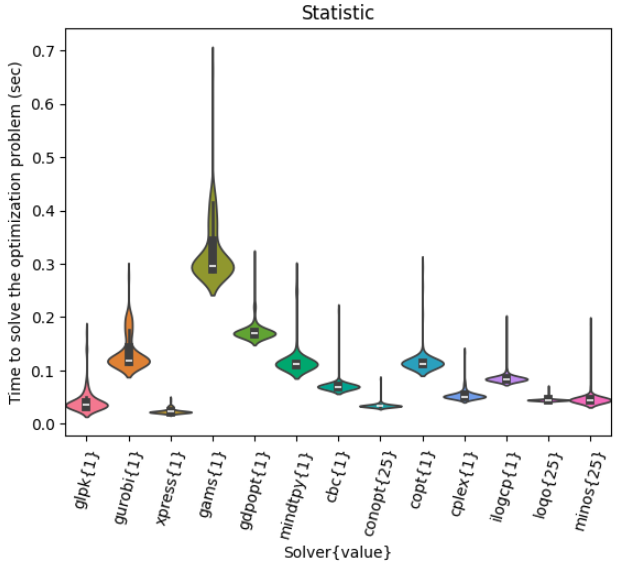
\includegraphics[width=1\textwidth]{solution}
  \caption{Результаты экспериментов}
  \label{fig:solution}
\end{figure}

\subsection*{Анализ результатов экспериментов}
Результаты экспериментов показывают, что время, потребное различным решателям для вычисления одних и тех же параметров может отличаться в разы. А так же, что нельзя идентифицировать полученный ответ от решателя как единственно верный. Лучше проводить серию экспериментов с разными решателями для получения достоверного результата.

Наименьшее значение результирующей стоимости, которое было достигнуто решателями, составляет $1$. Это значение было достигнуто $10$-ю решателями из $12$. А наибольшее значение стоимости составляет $25$ и оно получилось в результате работы $2$-х решателей: \textit{conopt} и \textit{minos}. Наименьшее медианное время, потребное для вычислений, показали решатели \textit{glpk}, \textit{xpress} и \textit{conopt}. Наибольшее время потребовалось решателю \textit{gams}.
